% !TeX spellcheck = en_US
% !TeX encoding = utf8
% !TeX program = xelatex
% !BIB program = bibtex

\documentclass[12pt]{article}
	\usepackage{amsmath,amssymb,amsfonts}
	\usepackage{latexsym}
	\usepackage{graphicx}
	\usepackage{verbatim}
	\usepackage{booktabs}
	\usepackage[usenames,dvipsnames,svgnames,table]{xcolor}
	\usepackage{todonotes} % Required for the boxes that questions appear in

	\newcommand{\mybox}[1]
	{
	\par\noindent
	\todo[inline, backgroundcolor=SkyBlue!40,bordercolor=SkyBlue,size=\large]{\textbf{#1}}
	
	}

	\usepackage[top=25mm, bottom=25.4mm, left=16.7mm, right=18.9mm]{geometry}

	\usepackage{fancyhdr}
	\pagestyle{fancy}
	\lhead{Linear Optimization Assignment \#1}
	\chead{}
	\rhead{Due: Sunday, April 1}
	\renewcommand{\headrulewidth}{0.3pt}

	% \usepackage[framed,numbered,autolinebreaks,useliterate,final]{mcode}
	\usepackage{listings}
	\title{\textbf{Linear Optimization Assignment \#1}}
	\author{Due: Sunday, April 1}
	\date{}

	\makeatletter
	\def\@seccntformat#1{%
		\expandafter\ifx\csname c@#1\endcsname\c@section\else
		\csname the#1\endcsname\quad
		\fi}
	\makeatother

	\usepackage{multirow}

	\usepackage{sectsty}
	\sectionfont{\color{NavyBlue}\selectfont}
	\subsectionfont{\color{SkyBlue}\itshape\selectfont}

	\newcommand{\abs}[1]{\left| #1 \right| }
	\newcommand{\norm}[1]{\left\| {#1} \right\|}

	% \setlength{\parsep}{0em}
	\setlength{\parskip}{.33em}
	\setlength{\parindent}{0em}	

\begin{document}
\maketitle

\textbf{\color{NavyBlue}Instruction:} Write a report and complete code. Upload them to ftp.
\begin{itemize}
	\item Upload:  \\
	      - Address: 10.13.72.84 \\
	      - Username: opt; Passwd:  opt18; Port: 21
	\item Download: \\
	      - Address: 10.13.71.168 \\
	      - Username: opt; Passwd:  opt18; Port: 21
\end{itemize}


% \begin{abstract}
% 	Enter a short summary here. What topic do you want to investigate and why? What experiment did you perform? What were your main results and conclusion?
% \end{abstract}

\section{Problem 1}

A McCulloch-Pitts (M-P) neuron accepts bipolar input $x_i \in \{-1,1\}$ and gives  $y=\mathrm{sgn} (\sum_{i=1}^{m} w_ix_i + b) $.

Give weights and bias for a M-P neuron with inputs
$x,y,z \in \{-1,1\}$ and whose output is  $z$ if $x = -1$ and $y = 1$, and is $-1$ otherwise.


% \section{Problem 2.}
% The following figure shows the decision regions of four classes. Design a
% classifier for these linearly inseparable classes, using a network consists of M-P neurons with
% three output units. For class $i$ $(1 \le i \le 3)$, classification requires that $y_i = 1$, with $y_j = -1$ for
% $j \ne i$. Class 4 is recognized when $y_i = -1$ for $1 \le i \le 3$.

% \begin{figure}[!htbp]
% 	\centering
% 	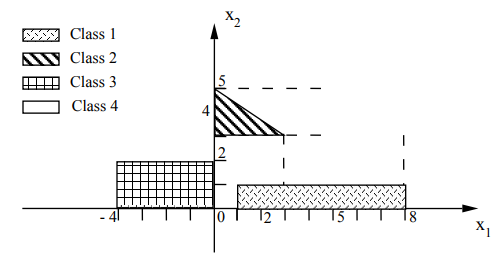
\includegraphics[width=0.7\textwidth]{fig/2018-03-17-14-09-07.png}
% \end{figure}

\section{Problem 2: Gradient Descent} 
SGD has trouble navigating ravines, i.e. areas where the surface curves much more steeply in one dimension than in another, which are common around local optima. Momentum is a method that helps accelerate SGD in the relevant direction and dampens oscillations as can be seen in fig~\ref{fig:momentum}. 

\begin{eqnarray*}
	v_t & = & \mu v_{t-1} + \varepsilon \nabla_\theta J(\theta)  \\ 
	\theta & =& \theta - v_t 
\end{eqnarray*}

\begin{figure}[!htbp]
	\centering 
	
\includegraphics[width=.7\textwidth]{fig/2018-03-19-13-38-08.png}
	\caption{Left: SGD without momentum; Right: SGD with momentum} \label{fig:momentum}
\end{figure}


\begin{description}
	\item[a).] Execute four iterations of gradient descent with momentum to find the minimum of
	the function $f(u) = \frac{u^3}{3} + 50 u^2-100u-30$. Start with $u = 20$, use a learning rate
	that is set to $\varepsilon = 0.01$, and parameter $\mu$ set to $0.1$.
	\item[b).] Evaluate the benefit of using a momentum for the task in a). by comparing your
	findings to the vanilla gradient descent method.
\end{description}

\section{Problem 3: Forward-Backward-Pass} 
Examine the multi-layer perceptron given in fig~\ref{fig:mlp}.

\begin{figure}[!htbp]
	\centering
	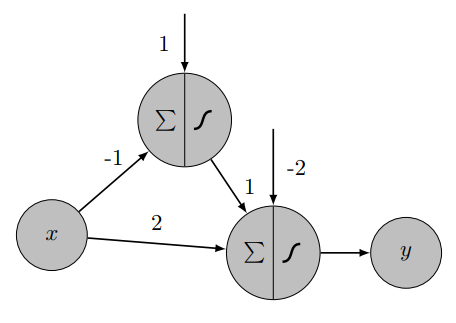
\includegraphics[width=.5\textwidth]{fig/2018-03-19-13-49-49.png}
	\caption{MLP with two logistic units} \label{fig:mlp}
\end{figure}

\begin{description}
\item[a).]	Both neurons use the logistic activation function 
$f(u)=\frac{1}{1+e^{-u}}$
The network has 
a single input variable $x$ and one output variable $y$. Calculate the output of both
neurons and the error made by the MLP when applying a pattern with $x = 0$ and
target value $0.5$.
\item[b).] Calculate the partial derivatives of the error with respect to the weights for the
pattern used in task a). 
\end{description}

\section{Problem 4: Multi-Layer Perceptron Architecture}

\begin{figure}[!htbp]
	\centering
	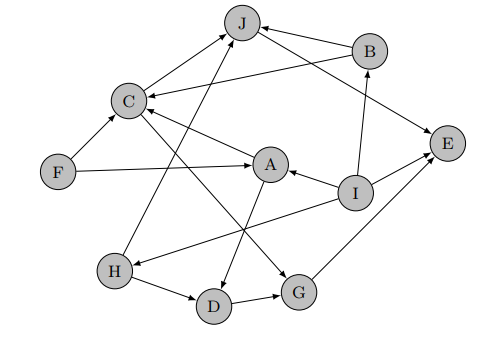
\includegraphics[width=.55\textwidth]{fig/2018-03-19-13-54-31.png}
	\caption{MLP with ten neurons} \label{fig:mlp2} 
\end{figure}

Now, consider the network structure of a multi-layer perceptron with 10 neurons given in
fig~\ref{fig:mlp2}. Each circle denotes a neuron, the arrows denote connections between neurons.
\begin{description}
	\item[a).]  Which of the neurons are input neurons, which ones are output neurons?
	\item[b).] How many layers does this MLP have? Which neurons belong to which layer?
	\item[c).] Assume we are applying a pattern to the MLP. Give an order in which the neuron
	activations $a_i$ can be calculated.
\end{description}

\section{Problem 5: Multi-Layer Perceptrons}

Which of the functions given by the plots in fig~\ref{fig:mlp3} can be implemented by multi-layer
perceptrons? The MLP should only contain neurons with logistic activation functions.
(Note: The weights of the networks must be finite numbers.)

\begin{figure}
	\centering 

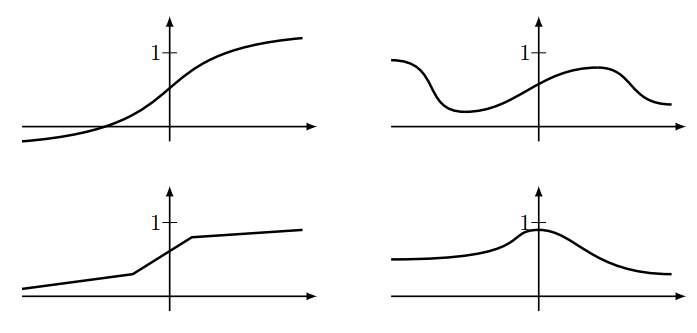
\includegraphics[width=.75\textwidth]{fig/2018-03-19-13-57-32.png}
\caption{Functions to be realized by MLPs} \label{fig:mlp3} 
\end{figure}


\section{Problem 6: MLP and BackPropogation} \label{sec:3}

\begin{itemize}
	
	\item Download ``hw2.zip'', The code pass test under Python 2.7.14 and Python 3.6.3. Complete code surrounded by ``TODO'' in ``net.py'' and ``opt.py''. For example,
	      \begin{verbatim}
###########################################################################
# TODO: Implement the affine forward pass. Store the result in out. You   #
# will need to reshape the input into rows.                               #
###########################################################################


###########################################################################
#                             END OF YOUR CODE                            #
###########################################################################
	\end{verbatim}
	\item Run ``python main\_check.py'' and paste the settings (\textit{e.g.} random seed, loss function name) and the results to  your report.  Make sure your code pass gradient check, \textit{i.e.}, relative error between Numerical gradient and analytic gradient is small (\textit{e.g.} smaller than 1e-7). We use centered formula $\displaystyle \frac{\mathrm{d}f(x)}{\mathrm{d}x} \approx \frac{f(x+h)-f(x)}{h}$ to compute numerical gradient since it has an error on order of $O(h)$ and use relative error as metric.
	\item Run ``python main\_train.py'' to train a model on fake data. 
	\item Do something extra surrounding the topics in this assignment,  using the code you developed. For example, is there some other interesting question we could have asked? Is there any insightful visualization you can plot? We did not use large cifar10 data. You can select some samples (\textit{e.g.} 50 or 500) in cifar10 or use the dataset in Problem~\ref{sec:4} to do real case analysis.
	\item You do not necessarily strictly use the framework provided by teacher assistant. You can use any language and framework and write from scratch.
	 Even tensorflow/pytorch with autograd is permitted, if you have time. 
	  Just make sure implement MLP by yourself and then do similar experiments, \textit{i.e.}, do not use any function like MLP or LinearRegression.  
\end{itemize}



\section{Problem 7: Predict House Prices} \label{sec:4}
Given 79 explanatory variables describing (almost) every aspect of residential homes, such as the size  and the location of the house, please predict the final price of each home.

\begin{itemize}

	\item The dataset is cleaned to become simple train/val format. You can try to modify the process of data clean.
	\item Make sure implement the regression model by yourself and do not use something like LinearRegression.  Regression is similar to MLP, which have been implemented in  Problem~\ref{sec:3}.

	\item Encourage to do model selection. For example, try lasso regression, humble loss or learning rate decay and select best model by cross validation. 

	\item You do not necessarily strictly use the framework provided by teacher assistant. You can use any language and write from scratch. Just make sure implement regression model by yourself and then do similar experiments. 
\end{itemize}

\end{document}

